\documentclass{../avaliacao}

% TODO: ajustar o codigo/nome da disciplina antes de usar de verdade
\configuraavaliacao
  {ITec - Instituto de Tecnologia}
  {XXXXX}
  {Automação Industrial}
  {Júlio Santos}
  {Avaliação \#1 -- Parte Teórica}
  {outubro de 2026}
  {../../logo_upf.png}

% Para imprimir o gabarito junto da prova, descomente a linha abaixo:
% \printanswers

\begin{document}

\imprimecabecalho

\begin{center}
\textbf{Instruções:} prova individual, \textbf{sem consulta}. Duração: 19h20 às 20h45 (85 min).
\end{center}
\vspace{0.5cm}

\begin{questions}

% Espaco de resposta proporcional ao tamanho esperado da resposta --
% ajuste os valores abaixo depois de ver a paginacao real compilada.
% Tema: introducao ao CLP (aula 01)
\question[2] O que é o \textbf{ciclo de varredura} (\textit{scan cycle}) de um CLP? Cite as três etapas básicas que se repetem a cada ciclo.

\begin{solution}
O ciclo de varredura é a sequência repetida de operações que o CLP executa continuamente durante a operação:
\begin{enumerate}
  \item \textbf{Leitura das entradas} -- o CLP lê o estado de todas as entradas físicas e grava numa tabela/imagem de entrada.
  \item \textbf{Execução do programa} -- o programa (Ladder/ST/...) é executado do início ao fim, usando os valores lidos.
  \item \textbf{Escrita das saídas} -- os valores calculados são escritos de uma vez nas saídas físicas.
\end{enumerate}
Esse ciclo se repete indefinidamente, com um tempo de varredura tipicamente da ordem de poucos milissegundos.
\end{solution}

\vspace{3.5cm}
% Tema: Ladder basico, portas logicas (aulas 02/03)
\question[4] Descreva (em palavras ou desenhando) o rung em Ladder de uma saída \texttt{Q} que liga quando os contatos \texttt{A} \textbf{E} \texttt{B} estiverem fechados, mas \textbf{não} liga quando \texttt{C} estiver fechado.

\begin{solution}
Um rung com \texttt{A} e \texttt{B} em série (dois contatos NA), e um contato \texttt{C} também em série mas do tipo NF (normalmente fechado), todos alimentando a bobina \texttt{Q}:
\begin{center}
\texttt{---| A |---| B |---|/C|---( Q )---}
\end{center}
Lógica equivalente: $Q = A \cdot B \cdot \overline{C}$.
\end{solution}

\vspace{3.5cm}
% Tema: partida de motor / hardware (aula 04)
\question[3] Por que a saída digital (GPIO) de um microcontrolador nunca deve acionar diretamente a bobina de um contator? O que deve ser colocado entre os dois?

\begin{solution}
A bobina de um contator normalmente opera em tensão/corrente muito maior do que uma GPIO consegue fornecer (a GPIO tipicamente fornece poucos miliampères em 3,3V/5V), e contatores geram picos de tensão indutivos ao desenergizar, que podem danificar o microcontrolador. Por isso, usa-se um \textbf{módulo relé isolado (opto-acoplado)} entre a GPIO e a bobina do contator: a GPIO aciona a bobina de baixa potência do relé, e os contatos do relé (eletricamente isolados) fecham o circuito de potência que energiza o contator.
\end{solution}

\vspace{2.5cm}
% Tema: partida de motor / hardware (aula 04)
\question[3] Por que um botão ligado a uma entrada digital que não tem resistor de pull interno precisa de um resistor de pull-down (ou pull-up) externo?

\begin{solution}
Sem um resistor de pull, quando o botão está solto a entrada fica ``flutuando'' (não conectada firmemente nem ao nível alto nem ao baixo), captando ruído eletromagnético do ambiente e podendo ler valores aleatórios e instáveis. O resistor de pull-down (ligado ao GND) ou pull-up (ligado à alimentação) garante um nível lógico definido quando o botão está solto, e o botão, ao ser pressionado, sobrepõe esse nível com o oposto.
\end{solution}

\vspace{2.5cm}
% Tema: bordas, set/reset, temporizadores (aula 06)
\question[2] Por quanto tempo, no máximo, um contato de detecção de borda de subida (\texttt{P}) permanece em nível \texttt{1}?

\begin{solution}
Apenas \textbf{um ciclo de varredura} (scan), independentemente de quanto tempo o sinal de entrada permanecer em \texttt{1} depois da transição.
\end{solution}

\vspace{2cm}

\newpage
% Tema: bordas, set/reset, temporizadores (aula 06)
\question[6] A figura abaixo mostra o sinal de entrada \texttt{IN} de dois temporizadores ao longo do tempo, com o tempo programado \texttt{PT} indicado. Desenhe, nos espaços abaixo do sinal \texttt{IN}, a saída \texttt{Q} de um bloco \texttt{TON} e de um bloco \texttt{TOF}, ambos recebendo esse mesmo \texttt{IN} e o mesmo \texttt{PT}.

\begin{center}
\begin{tikzpicture}[scale=1]
  \draw[thick] (0,0) node[left] {IN} -- (1,0) -- (1,1) -- (4,1) -- (4,0) -- (8,0);
  \draw[dashed] (1,0) -- (1,-3.5);
  \draw[dashed] (2.5,0) -- (2.5,-3.5);
  \draw[dashed] (4,0) -- (4,-3.5);
  \draw[<->] (1,1.4) -- (2.5,1.4);
  \node[above] at (1.75,1.4) {PT};

  \node[left] at (0,-0.7) {Q (TON)};
  \draw[gray] (0,-1) -- (8,-1);

  \node[left] at (0,-2.7) {Q (TOF)};
  \draw[gray] (0,-3) -- (8,-3);

  \draw[->] (8,0) -- (8.3,0) node[right] {t};
\end{tikzpicture}
\end{center}

\begin{solution}
\begin{center}
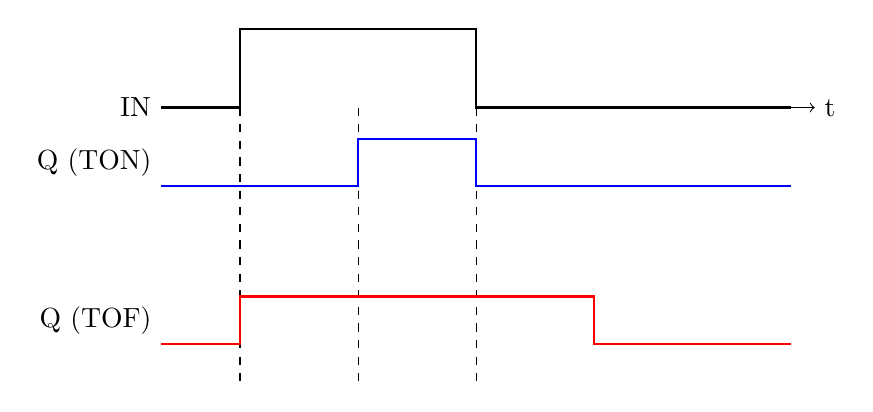
\begin{tikzpicture}[scale=1]
  \draw[thick] (0,0) node[left] {IN} -- (1,0) -- (1,1) -- (4,1) -- (4,0) -- (8,0);
  \draw[dashed] (1,0) -- (1,-3.5);
  \draw[dashed] (2.5,0) -- (2.5,-3.5);
  \draw[dashed] (4,0) -- (4,-3.5);

  \node[left] at (0,-0.7) {Q (TON)};
  \draw[thick, blue] (0,-1) -- (2.5,-1) -- (2.5,-0.4) -- (4,-0.4) -- (4,-1) -- (8,-1);

  \node[left] at (0,-2.7) {Q (TOF)};
  \draw[thick, red] (0,-3) -- (1,-3) -- (1,-2.4) -- (5.5,-2.4) -- (5.5,-3) -- (8,-3);

  \draw[->] (8,0) -- (8.3,0) node[right] {t};
\end{tikzpicture}
\end{center}
O \texttt{TON} atrasa a \textbf{subida} de \texttt{Q} em \texttt{PT} depois que \texttt{IN} sobe, e desce imediatamente quando \texttt{IN} cai. O \texttt{TOF} sobe imediatamente junto com \texttt{IN}, e atrasa a \textbf{descida} de \texttt{Q} em \texttt{PT} depois que \texttt{IN} cai.
\end{solution}

\vspace{1cm}

\newpage
% Tema: bordas, set/reset, temporizadores (aula 06)
\question[4] As bobinas Set (\texttt{S}) e Reset (\texttt{R}) do mesmo bit são ativadas ao mesmo tempo, no mesmo ciclo de varredura. Qual o valor final do bit, e como isso é decidido, pensando em Ladder (não em código)?

\begin{solution}
Quem ``vence'' é a bobina do \textbf{rung que for resolvido por último} -- o CLP executa os rungs de cima para baixo, na ordem em que aparecem no programa. Se o rung de Reset vier depois do rung de Set, o Reset prevalece (``Reset dominante''); se o Set vier depois, o Set prevalece. Não há uma regra fixa da norma para Ladder -- depende da ordem em que o programador colocou os rungs.
\end{solution}

\vspace{2.5cm}
% Tema: bordas, set/reset, temporizadores (aula 06)
\question[2] Que tipo de variável da norma IEC 61131-3 é usado no parâmetro \texttt{PT} de um temporizador? Dê um exemplo de literal válido para esse tipo.

\begin{solution}
O tipo é \texttt{TIME}. Exemplo de literal válido: \texttt{T\#2s500ms} (2,5 segundos), ou \texttt{T\#1h30m} -- sempre prefixado por \texttt{T\#}, combinando dias/horas/minutos/segundos/milissegundos.
\end{solution}

\vspace{2cm}
% Tema: variaveis no OpenPLC (aula 07)
\question[3] Diferencie os endereços \texttt{\%IX0.0}, \texttt{\%QW0} e \texttt{\%MW3}.

\begin{solution}
\begin{itemize}
  \item \texttt{\%IX0.0} -- entrada (\texttt{I}) digital/booleana (\texttt{X}), byte 0, bit 0.
  \item \texttt{\%QW0} -- saída (\texttt{Q}) do tipo palavra/\texttt{WORD} (\texttt{W}), posição 0 -- por exemplo, uma saída analógica.
  \item \texttt{\%MW3} -- memória interna (\texttt{M}) do tipo palavra (\texttt{W}), posição 3 -- uma variável interna do programa, sem ligação direta com E/S física.
\end{itemize}
\end{solution}

\vspace{2.5cm}

\newpage
% Tema: variaveis no OpenPLC (aula 07)
\question[4] Uma entrada analógica bruta chega como um valor inteiro de 0 a 65535 (\texttt{WORD}). Explique (com fórmula ou raciocínio) como converter essa leitura para uma faixa de 0 a 100 (percentual).

\begin{solution}
Basta uma regra de três simples:
\[
\text{percentual} = \text{leitura} \times \dfrac{100}{65535}
\]
Ou seja, dividir o valor bruto pelo valor máximo possível (65535) e multiplicar por 100, mapeando linearmente a faixa 0--65535 para 0--100.
\end{solution}

\vspace{2.5cm}
% Tema: termostato simulado (aula 08)
\question[3] O que é histerese (banda morta) num controle liga/desliga, e que problema ela evita?

\begin{solution}
Histerese é usar dois limiares diferentes -- um para ligar e outro, mais afastado, para desligar -- em vez de um único limiar. Isso evita que a saída fique ``tremendo'' (ligando e desligando repetidamente, muito rápido) quando a variável controlada oscila bem perto de um único limiar.
\end{solution}

\vspace{2cm}
% Tema: termostato simulado (aula 08)
\question[3] Por que um motor ou compressor deveria ter um tempo mínimo de bloqueio antes de poder religar, depois de ter desligado?

\begin{solution}
Religar um motor/compressor rapidamente demais depois de desligar pode causar desgaste mecânico e elétrico prematuro (esforço extra no religamento, picos de corrente de partida muito seguidos), reduzindo a vida útil do equipamento. O bloqueio (tempo mínimo desligado) evita esse ciclo curto de liga-desliga.
\end{solution}

\vspace{2cm}

\tabelapontuacao

\end{questions}

\end{document}
